\chapter{Justificación del diseño y consideraciones técnicas fundamentales}
\label{cap:JustificacionYConsideraciones}
En este capítulo se han desarrollado en profundidad tanto los aspectos técnicos del proyecto como las decisiones que se han tomado en cuanto al rumbo a seguir de la aplicación en distintos niveles.
\section{Código abierto}
El código libre o abierto
\footnote{La mayoría del contenido en este apartado ha tomado las referencias del libro The innovators \citep{Innovators}} 
(significando esto que el código desarrollado está público para cualquiera que lo quiera ver)
es un movimiento socio-tecnólogico que comenzó en la decada de 1980, cuando Richard Stallman (considerado por muchos el padre del movimiento de código abierto) fundó la \href{https://www.fsf.org/}{\textit{Free Software Foundation}}, así como el sitema operativo \href{https://www.gnu.org/}{GNU} (\textit{GNU's not Unix}), este creía que el software se tendría que crear de forma colaborativa y libremente compartido. Otro gran exponente de este movimiento (aunque con distintas motivaciones) fue el finlandés Linus Torwalds, creador del kernel Linux (GNU-Linux es el sistema operativo con el que se está escribiendo esta memoria y se ha realizado todo el proceso de desarrollo).

En este contexto, se ha intentado desarrollar Profinder siguiendo estos principios e intentando utilizar la mayor cantidad de herramientas de código abierto posible. Algunos ejemplos a parte de los que se han ido mencionando a lo largo de esta memoria pueden ser \href{https://www.mozilla.org/es-ES/firefox/}{Firefox}, \href{https://neovim.io/}{Neovim} y \href{https://www.linux.org/pages/}{Linux} entre otros. Asimismo se ha decidido que todo el código de este proyecto sea libre -siendo posible revisarlo, distribuirlo y modificarlo- así como el proceso seguido para hacerlo.

\section{Idiomas}
El idioma principal utilizado para el desarrollo de Profinder (código, apuntes, \textit{commits}) ha sido el inglés con el objetivo de hacer el proyecto lo mas ‘universal’ posible, por tanto, el idioma original de la aplicación es el inglés. Sin embargo, se ha desarrollado de tal forma que también tiene una versión en español, de la misma forma podría ser traducida a cualquier otro idioma.

\section{Arquitectura y patrones}
\subsection{CLEAN architecture}
\label{subsec:cleanArch}
La arquitectura CLEAN, originaria del libro Clean architecture \citep{CleanArchitecture}, es una forma de estructurar el software, dividiendolo en distintas capas que abstraigan el código y separen responsabilidades. Gracias al uso de esta arquitectura, se ha podido crear un proyecto escalable y robusto. También se han ahorrado muchos dolores de cabeza en los distintos procesos de refactorización ya que al haber tenido una estructura ordenada y bien definida, se han evitado posibles efectos secundarios por causa de los distintos cambios.

En Profinder se ha adaptado esta arquitectura a la programación en Android, dividiéndose así el código en cuatro capas explicadas a continuación:
\begin{enumerate}
    \item core: en esta capa van los recursos comunes que pueden ser accedidos por todas las demás capas, esta es una relación unidireccional ya que core no puede acceder a las demás capas. En este proyecto en particular se ha utilizado para guardar todo el boilerplate necesario para la aplicación del MVI (explicado en la apartado \ref{subsec:mvi}), modelos de datos para pruebas, y utilidades como la clase encargada de formatear las fechas y cominar los identificadores de usuarios.
    \item data: en esta capa es donde se gestionan todos los servicios y se preparan para ser enviados a la capa domain (explicada en el siguiente punto). Esta capa tiene toda la lógica de aplicación y es la encargada de decidir de dónde sacar los datos, todas las llamadas de red se hacen en esta capa. En muchos casos, esta capa tiene un modelo de datos propio (los datos tal cual llegan de los \textit{endpoints}) que adapta mediante el uso de \textit{mappers} para ser enviados a la siguiente capa.
    \item domain: En esta capa se encuentra la lógica de negocio de la aplicación, esta capa sería común a todas las versiones de la aplicación si se hicieran para otros sistemas operativos (IOS, Windows...) a excepción de la adecuación con el lenguaje de programación específico de cada sistema operativo, esto significa que no le ‘importa’ de donde vienen los datos, cuenta con una interfaz (denominada repositorio) en la que se ha definido el contrato con la capa de data y es ahí donde pide los datos que le deben llegar según su propio modelo de datos (mapeados). Es en esta capa donde se definen los casos de uso, que actúan como contratos entre la capa de UI (ecplicada en el siguiente punto) y el repositorio. Esta implementación abstrae responsabilidades y ayuda a la encapsulación. 
    \item ui: Esta es toda la capa de interfaz de usuario de la aplicación, realizada utilizando \hyperlink{subsec:compose}{Jetpack compose} y siguiendo el patrón arquitectónico  MVI (\ref{subsec:mvi}). Las vistas como tal (denominadas \textit{Composables}) se comunican con los casos de uso (capa domain) a través de unas clases denominadas \href{https://developer.android.com/topic/libraries/architecture/viewmodel}{\textit{Viewmodels}}.

\end{enumerate}
\subsection{MVI}
\label{subsec:mvi}
Debido a que en una aplicación móvil la mayor parte del trabajo se realiza en la interfaz de usuario, es habitual seguir patrones de diseño (mejor denominados: pseudo-arquitecturas). En el caso de Profinder había dos posibilidades: \href{https://builtin.com/software-engineering-perspectives/mvvm-architecture}{MVVM} (Model-View-Viewmodel) o MVI (Model-View-Intent). Se decidió seguir el patrón MVI por ser más organizado y viable para aplicaciones de tamaño grande, a su vez es un patrón que se adapta muy bien al paradigma de programación en kotlin (programación funcional), su única desventaja es que introduce código de relleno para la estructuración (denominado boilerplate), pero esto a su vez ayuda a que sea más entendible por terceros a medida que aumenta el tamaño del proyecto. A continuación se explica en qué consiste esta pseudo-arquitectura y como se ha aplicado en el proyecto:
\begin{itemize}
    \item \textbf{Model}: es un término que puede variar en distintas pseudo-arquitecturas, en MVI es el que representa el estado de los datos, es inmutable y cuando se quiere cambiar algún atributo se destruye y se vuelve a crear con las nuevas modificaiones, esto ayuda a aumentar la testabilidad del código. Por ejemplo podemos tener un estado para la carga de datos (una  variable loading) y otro para el usuario (empieza siendo nulo y cuando se han cargado los datos se reescribe el estado con la nueva variable).
    \begin{figure}[h]
        \centering
        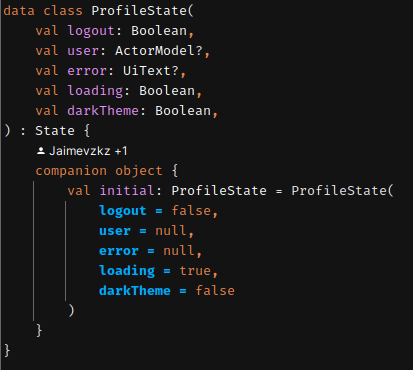
\includegraphics[width = 0.7\textwidth]{Imagenes/Fuentes/ejemplo_estado.png}
        \caption{Ejemplo de estado.}
        \label{fig:ejemplo_estado}
    \end{figure}
    \item \textbf{View}: se encarga de observar el estado y renderizar en la vista de forma reactiva. Por ejemplo, en el caso de observar que cambia el valor de la variable loading, dibujaríamos un shimmer (pantalla de carga), y cuando el valor de loading se pusiera a \textit{true} y tras comprobar que no hubiera errores, se dibujaría la vista como tal. Esto hace que la vista sea ‘tonta’ en el sentido de que no tiene que tomar ningún tipo de decisión, solo recibe unos datos en el estado y los pinta.
    \item \textbf{Intent}: se define como una acción (No confundir con \href{https://developer.android.com/guide/components/intents-filters}{Intent de Android}) que se lanza cuando el usuario realiza una acción (o el sistema solicita un cambio de estado). Estas acciones se procesan en un \textit{pipe} del viewmodel y van sobreescribiendo el estado. Es la forma que tiene la vista de cambiar los datos, cuando el usuario realiza una opción (como por ejemplo pulsar un botón), la vista lanza un \textit{intent} que se procesa, haciendo los cambios de estado necesarios.
    \begin{figure}[h]
        \centering
        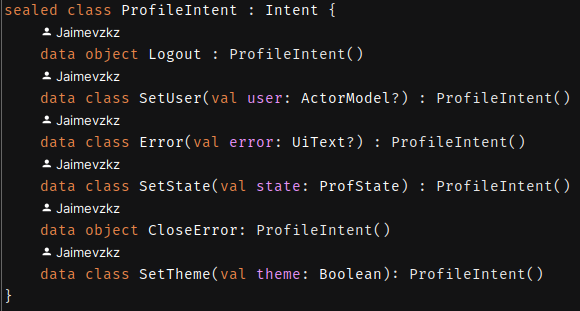
\includegraphics[width = 0.7\textwidth]{Imagenes/Fuentes/ejemplo_intent.png}
        \caption{Ejemplo de definición de los \textit{intents} de una vista.}
        \label{fig:ejemplo_intent}
    \end{figure}
\end{itemize}
Esta estructura define un flujo unidireccional de datos: La vista lanza intents que sobreescriben el estado, como consecuencia de este cambio de estado cambia la vista. Este flujo tiene muchas ventajas que ayudan a crear un código entendible, organizado y escalable.
\begin{figure}[h]
    \centering
    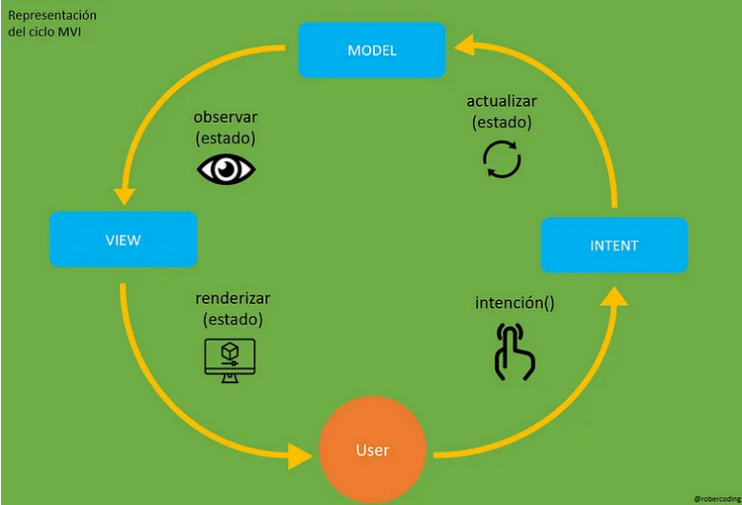
\includegraphics[width = 0.5\textwidth]{Imagenes/Fuentes/visual_mvi.png}
    \caption{Representación gráfica del ciclo MVI \citep{mviExplanation}.}
    \label{fig:visualMvi}
\end{figure}

\subsection{Principios SOLID}
Los principios SOLID son un conjunto de cinco principios de diseño de software que fueron introducidos en el libro Clean Code \citep{CleanCode}. Están destinados a guiar a los desarrolladores hacia la creación de código fuente limpio, modular, mantenible y extensible. A continuación se ha descrito brevemente cada uno de ellos, adjuntando una captura del código de la aplicación que lo implementa o una explicación de en qué parte del código se ha implementado cuando lo anterior no sea posible:
\begin{enumerate}
    \item Principio de Responsabilidad Única (\textit{Single Responsibility Principle}): establece que una clase debería tener una única razón para cambiar. En otras palabras, una clase debe tener una sola responsabilidad o función dentro del sistema. En el ejemplo, cualquier clase que implemente la interfaz tendrá la responsabilidad única de implementar el metodo \textit{invoke}.
    \begin{figure}[h]
        \centering
        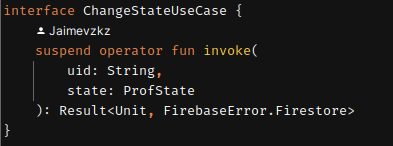
\includegraphics[width = 0.7\textwidth]{Imagenes/Fuentes/change_state.png}
        \caption{Ejemplo de primer principio SOLID.}
        \label{fig:change_state}
    \end{figure}
    \item Principio de Abierto/Cerrado (\textit{Open/Closed Principle}): sostiene que las entidades de software (clases, módulos, funciones, etc.) deberían estar abiertas para su extensión pero cerradas para su modificación.
    
    Este principio se podría ver implementado por ejemplo en la funcionalidad \textit{profile}, en la que se podría añadir todo el código que se deseara para añadir funcionalidad sin tener que cambiar nada de lo ya implementado.
    \item Principio de Sustitución de Liskov (\textit{Liskov Substitution Principle}): establece que los objetos de un programa deben ser reemplazables por instancias de sus subtipos sin afectar la integridad del programa.
    
    En Profinder, este principio ha sido implementado por ejemplo en los \textit{viewmodels}, que heredan de la clase \textit{Baseviewmodel}. Cualquier instancia del objeto \textit{Baseviemodel} podría ser sustituido por la implementación una de alguna de sus clases hijas sin que cambiara el comportamiento del programa.
    \item Principio de Segregación de la Interfaz (\textit{Interface Segregation Principle}):  sostiene que es mejor el uso de muchas interfaces pequeñas y concretas, mejor que una monolítica para evitar dependencias innecesarias.
    
    Esto se aplica en los casos de uso, cada caso de uso tiene una interfaz específica y concreta.
    \item Principio de Inversión de Dependencias (\textit{Dependency Inversion Principle}): establece que los módulos de alto nivel no deben depender (ni al revés) de los módulos de bajo nivel, ambos deben depender de abstracciones.
    
    Esto se cumple por ejemplo en la implementación \textit{reduce} de los viewmodel, esta función no tiene ninguna dependecia específica de la que dependa, sino que se adapta a cada caso recibiendo tipos genéricos.
    \begin{figure}[h]
        \centering
        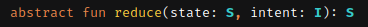
\includegraphics[width = 0.7\textwidth]{Imagenes/Fuentes/ejemplo_reduce.png}
        \caption{Ejemplo del quinto principio SOLID.}
        \label{fig:ejemplo_reduce}
    \end{figure}
\end{enumerate}

\section{Gestión de errores} 
Para conseguir una gestión de errores eficiente y generalizada que ayudara a encontrar errores se han desarrollado una serie de clases
\footnote{Este sistema de gestión de errores se ha realizado siguiendo el propuesto en este tutorial: \href{https://www.youtube.com/watch?v=MiLN2vs2Oe0}{Philipp Lackner on Error handling} y ha sido personalizado según las necesidades específicas de la aplicación.}
que en conjunto sirven como sistema bien estructurado que proporciona una forma cómoda de gestionar errores, respetando todos los principios de arquitectura limpia menciandos en el apartado \ref{subsec:cleanArch}. A continuación se explican todas las clases que se han creado, es posible que solo con la explicación que viene a continuación no se entiende el sistema en su totalidad, pero el lector tendrá disponible el código fuente para verlo aplicado y si es necesario clonar el repositorio para probarlo haciendo cambios.

En primer lugar se ha creado la interfaz \textit{Error} que no hará nada pero servirá para identificar todos los tipos de errores declarados.
\begin{figure}[h]
    \centering
    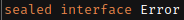
\includegraphics[width = 0.3\textwidth]{Imagenes/Fuentes/error_interface.png}
    \caption{Interfaz Error.}
    \label{fig:error_interface}
\end{figure}
En segundo lugar se ha creado la interfaz Result (se ha llamado así a pesar de que ya haya una clase con este nombre en la biblioteca estandar por considerarse el más apropiado). Esta es la interfaz principal que utilizan todas las funciones de la aplicación que devuelvan datos. Tiene dos parametros genéricos que cambiarán en cada caso específico, uno para los datos devueltos y otro para el tipo de error, también cuenta con los dos posibles resultados que pueda devolver una función que implemente esta interfaz: 
\begin{itemize}
    \item \textbf{Success}: para el caso de éxito. Llevará como parámetro los datos devueltos.
    \item \textbf{Error}: distinta de la interfaz explicada anteriormente, será lo que se devuelva en caso de error en la llamada a función y llevará como parámetro una clase que implemente la interfaz \textit{Error}.
\end{itemize}
\newpage
\begin{figure}[h]
    \centering
    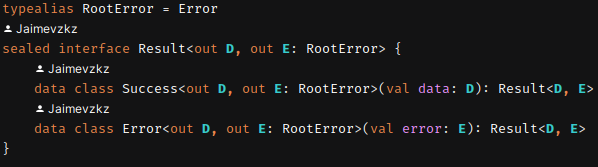
\includegraphics[width = 1\textwidth]{Imagenes/Fuentes/ejemplo_result.png}
    \caption{Interfaz Result.}
    \label{fig:ejemplo_result}
\end{figure}
\textbf{Result} y \textbf{Error} son las interfaces base del sistema. Lo siguiente será crear todas las interfaces que sean necesarias -e implementen \textit{Error}- para cada tipo de error. En Profinder solo ha sido necesario crear una que englobara todos los errores relativos a \hyperlink{subsec:firebase}{Firebase} ya que no ha habido necesidad de crear más, en cualquier caso, es un sistema escalable a futuro para múltiples tipos de errores.

Dentro de esta interfaz se declaran todos los tipos de errores (relativos a \hyperlink{subsec:firebase}{Firebase}, por ejemplo) como clases enumeradas, consiguiendo así que cada uno sea un enumerado que se gestiona de forma independiente en las distintas capas de la aplicación.
\begin{figure}[h]
    \centering
    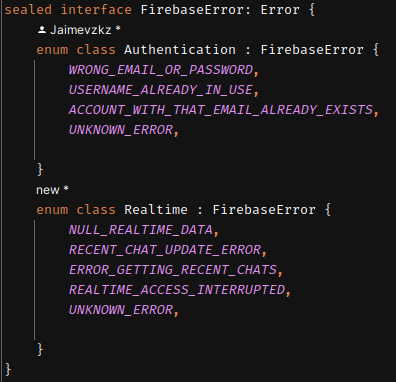
\includegraphics[width = 0.7\textwidth]{Imagenes/Fuentes/ejemplo_tipo_error.png}
    \caption{Ejemplo de tipo de error.}
    \label{fig:ejemplo_tipo_error}
\end{figure}

Con todo lo anterior, la gestión de errores se convierte en algo sencillo, las funciones deberán devolver un tipo \textit{Result}:
\newpage
\begin{figure}[h]
    \centering
    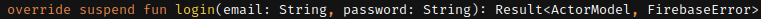
\includegraphics[width = 1\textwidth]{Imagenes/Fuentes/ejemplo_impl_result.png}
    \caption{Ejemplo de implementación de Result.}
    \label{fig:ejemplo_impl_result}
\end{figure}

Y en las llamadas a función se podrá gestionar si hay un error dividiendo los casos con una expresión \href{https://kotlinlang.org/docs/control-flow.html#when-expression}{\textit{when}}:
\begin{figure}[h]
    \centering
    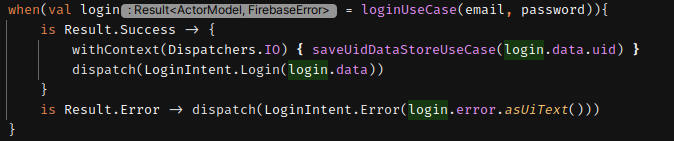
\includegraphics[width = 1\textwidth]{Imagenes/Fuentes/llamada_funcion_result.png}
    \caption{Ejemplo de llamada a función implementando Result.}
    \label{fig:llamada_funcion_result}
\end{figure}